\documentclass[twoside]{book}

% Packages required by doxygen
\usepackage{fixltx2e}
\usepackage{calc}
\usepackage{doxygen}
\usepackage[export]{adjustbox} % also loads graphicx
\usepackage{graphicx}
\usepackage[utf8]{inputenc}
\usepackage{makeidx}
\usepackage{multicol}
\usepackage{multirow}
\PassOptionsToPackage{warn}{textcomp}
\usepackage{textcomp}
\usepackage[nointegrals]{wasysym}
\usepackage[table]{xcolor}

% Font selection
\usepackage[T1]{fontenc}
\usepackage[scaled=.90]{helvet}
\usepackage{courier}
\usepackage{amssymb}
\usepackage{sectsty}
\renewcommand{\familydefault}{\sfdefault}
\allsectionsfont{%
  \fontseries{bc}\selectfont%
  \color{darkgray}%
}
\renewcommand{\DoxyLabelFont}{%
  \fontseries{bc}\selectfont%
  \color{darkgray}%
}
\newcommand{\+}{\discretionary{\mbox{\scriptsize$\hookleftarrow$}}{}{}}

% Page & text layout
\usepackage{geometry}
\geometry{%
  a4paper,%
  top=2.5cm,%
  bottom=2.5cm,%
  left=2.5cm,%
  right=2.5cm%
}
\tolerance=750
\hfuzz=15pt
\hbadness=750
\setlength{\emergencystretch}{15pt}
\setlength{\parindent}{0cm}
\setlength{\parskip}{0.2cm}
\makeatletter
\renewcommand{\paragraph}{%
  \@startsection{paragraph}{4}{0ex}{-1.0ex}{1.0ex}{%
    \normalfont\normalsize\bfseries\SS@parafont%
  }%
}
\renewcommand{\subparagraph}{%
  \@startsection{subparagraph}{5}{0ex}{-1.0ex}{1.0ex}{%
    \normalfont\normalsize\bfseries\SS@subparafont%
  }%
}
\makeatother

% Headers & footers
\usepackage{fancyhdr}
\pagestyle{fancyplain}
\fancyhead[LE]{\fancyplain{}{\bfseries\thepage}}
\fancyhead[CE]{\fancyplain{}{}}
\fancyhead[RE]{\fancyplain{}{\bfseries\leftmark}}
\fancyhead[LO]{\fancyplain{}{\bfseries\rightmark}}
\fancyhead[CO]{\fancyplain{}{}}
\fancyhead[RO]{\fancyplain{}{\bfseries\thepage}}
\fancyfoot[LE]{\fancyplain{}{}}
\fancyfoot[CE]{\fancyplain{}{}}
\fancyfoot[RE]{\fancyplain{}{\bfseries\scriptsize Generated on Sun Jan 25 2015 13\+:41\+:00 for My Project by Doxygen }}
\fancyfoot[LO]{\fancyplain{}{\bfseries\scriptsize Generated on Sun Jan 25 2015 13\+:41\+:00 for My Project by Doxygen }}
\fancyfoot[CO]{\fancyplain{}{}}
\fancyfoot[RO]{\fancyplain{}{}}
\renewcommand{\footrulewidth}{0.4pt}
\renewcommand{\chaptermark}[1]{%
  \markboth{#1}{}%
}
\renewcommand{\sectionmark}[1]{%
  \markright{\thesection\ #1}%
}

% Indices & bibliography
\usepackage{natbib}
\usepackage[titles]{tocloft}
\setcounter{tocdepth}{3}
\setcounter{secnumdepth}{5}
\makeindex

% Hyperlinks (required, but should be loaded last)
\usepackage{ifpdf}
\ifpdf
  \usepackage[pdftex,pagebackref=true]{hyperref}
\else
  \usepackage[ps2pdf,pagebackref=true]{hyperref}
\fi
\hypersetup{%
  colorlinks=true,%
  linkcolor=blue,%
  citecolor=blue,%
  unicode%
}

% Custom commands
\newcommand{\clearemptydoublepage}{%
  \newpage{\pagestyle{empty}\cleardoublepage}%
}


%===== C O N T E N T S =====

\begin{document}

% Titlepage & ToC
\hypersetup{pageanchor=false,
             bookmarks=true,
             bookmarksnumbered=true,
             pdfencoding=unicode
            }
\pagenumbering{roman}
\begin{titlepage}
\vspace*{7cm}
\begin{center}%
{\Large My Project }\\
\vspace*{1cm}
{\large Generated by Doxygen 1.8.9.1}\\
\vspace*{0.5cm}
{\small Sun Jan 25 2015 13:41:00}\\
\end{center}
\end{titlepage}
\clearemptydoublepage
\tableofcontents
\clearemptydoublepage
\pagenumbering{arabic}
\hypersetup{pageanchor=true}

%--- Begin generated contents ---
\chapter{Namespace Index}
\section{Packages}
Here are the packages with brief descriptions (if available)\+:\begin{DoxyCompactList}
\item\contentsline{section}{\hyperlink{namespaceedytorobrazuinny}{edytorobrazuinny} }{\pageref{namespaceedytorobrazuinny}}{}
\end{DoxyCompactList}

\chapter{Hierarchical Index}
\section{Class Hierarchy}
This inheritance list is sorted roughly, but not completely, alphabetically\+:\begin{DoxyCompactList}
\item Action\+Listener\begin{DoxyCompactList}
\item \contentsline{section}{edytorobrazuinny.\+Main.\+Skaluj\+Obraz}{\pageref{classedytorobrazuinny_1_1_main_1_1_skaluj_obraz}}{}
\item \contentsline{section}{edytorobrazuinny.\+Main.\+Skaluj\+Obraz}{\pageref{classedytorobrazuinny_1_1_main_1_1_skaluj_obraz}}{}
\item \contentsline{section}{edytorobrazuinny.\+Main.\+Tekst\+Dodaj}{\pageref{classedytorobrazuinny_1_1_main_1_1_tekst_dodaj}}{}
\item \contentsline{section}{edytorobrazuinny.\+Main.\+Tekst\+Dodaj}{\pageref{classedytorobrazuinny_1_1_main_1_1_tekst_dodaj}}{}
\end{DoxyCompactList}
\item Change\+Listener\begin{DoxyCompactList}
\item \contentsline{section}{edytorobrazuinny.\+Main.\+Jasnosc\+Obrazu}{\pageref{classedytorobrazuinny_1_1_main_1_1_jasnosc_obrazu}}{}
\item \contentsline{section}{edytorobrazuinny.\+Main.\+Jasnosc\+Obrazu}{\pageref{classedytorobrazuinny_1_1_main_1_1_jasnosc_obrazu}}{}
\end{DoxyCompactList}
\item \contentsline{section}{edytorobrazuinny.\+edytorobrazu}{\pageref{classedytorobrazuinny_1_1edytorobrazu}}{}
\item J\+Frame\begin{DoxyCompactList}
\item \contentsline{section}{edytorobrazuinny.\+Main.\+Jasnosc\+Obrazu}{\pageref{classedytorobrazuinny_1_1_main_1_1_jasnosc_obrazu}}{}
\item \contentsline{section}{edytorobrazuinny.\+Main.\+Jasnosc\+Obrazu}{\pageref{classedytorobrazuinny_1_1_main_1_1_jasnosc_obrazu}}{}
\item \contentsline{section}{edytorobrazuinny.\+Main.\+Skaluj\+Obraz}{\pageref{classedytorobrazuinny_1_1_main_1_1_skaluj_obraz}}{}
\item \contentsline{section}{edytorobrazuinny.\+Main.\+Skaluj\+Obraz}{\pageref{classedytorobrazuinny_1_1_main_1_1_skaluj_obraz}}{}
\item \contentsline{section}{edytorobrazuinny.\+Main.\+Tekst\+Dodaj}{\pageref{classedytorobrazuinny_1_1_main_1_1_tekst_dodaj}}{}
\item \contentsline{section}{edytorobrazuinny.\+Main.\+Tekst\+Dodaj}{\pageref{classedytorobrazuinny_1_1_main_1_1_tekst_dodaj}}{}
\end{DoxyCompactList}
\item Key\+Adapter\begin{DoxyCompactList}
\item \contentsline{section}{edytorobrazuinny.\+Main.\+Skaluj\+Obraz.\+Key\+List}{\pageref{classedytorobrazuinny_1_1_main_1_1_skaluj_obraz_1_1_key_list}}{}
\item \contentsline{section}{edytorobrazuinny.\+Main.\+Skaluj\+Obraz.\+Key\+List}{\pageref{classedytorobrazuinny_1_1_main_1_1_skaluj_obraz_1_1_key_list}}{}
\end{DoxyCompactList}
\end{DoxyCompactList}

\chapter{Class Index}
\section{Class List}
Here are the classes, structs, unions and interfaces with brief descriptions\+:\begin{DoxyCompactList}
\item\contentsline{section}{\hyperlink{classedytorobrazuinny_1_1edytorobrazu}{edytorobrazuinny.\+edytorobrazu} }{\pageref{classedytorobrazuinny_1_1edytorobrazu}}{}
\item\contentsline{section}{\hyperlink{classedytorobrazuinny_1_1_main_1_1_jasnosc_obrazu}{edytorobrazuinny.\+Main.\+Jasnosc\+Obrazu} }{\pageref{classedytorobrazuinny_1_1_main_1_1_jasnosc_obrazu}}{}
\item\contentsline{section}{\hyperlink{classedytorobrazuinny_1_1_main_1_1_skaluj_obraz_1_1_key_list}{edytorobrazuinny.\+Main.\+Skaluj\+Obraz.\+Key\+List} }{\pageref{classedytorobrazuinny_1_1_main_1_1_skaluj_obraz_1_1_key_list}}{}
\item\contentsline{section}{\hyperlink{classedytorobrazuinny_1_1_main_1_1_skaluj_obraz}{edytorobrazuinny.\+Main.\+Skaluj\+Obraz} }{\pageref{classedytorobrazuinny_1_1_main_1_1_skaluj_obraz}}{}
\item\contentsline{section}{\hyperlink{classedytorobrazuinny_1_1_main_1_1_tekst_dodaj}{edytorobrazuinny.\+Main.\+Tekst\+Dodaj} }{\pageref{classedytorobrazuinny_1_1_main_1_1_tekst_dodaj}}{}
\end{DoxyCompactList}

\chapter{File Index}
\section{File List}
Here is a list of all files with brief descriptions\+:\begin{DoxyCompactList}
\item\contentsline{section}{\hyperlink{edytorobrazu_8java}{edytorobrazu.\+java} }{\pageref{edytorobrazu_8java}}{}
\item\contentsline{section}{Edytor\+Obrazu\+Inny/src/edytorobrazuinny/\hyperlink{_edytor_obrazu_inny_2src_2edytorobrazuinny_2edytorobrazu_8java}{edytorobrazu.\+java} }{\pageref{_edytor_obrazu_inny_2src_2edytorobrazuinny_2edytorobrazu_8java}}{}
\end{DoxyCompactList}

\chapter{Namespace Documentation}
\hypertarget{namespaceedytorobrazuinny}{}\section{Package edytorobrazuinny}
\label{namespaceedytorobrazuinny}\index{edytorobrazuinny@{edytorobrazuinny}}
\subsection*{Classes}
\begin{DoxyCompactItemize}
\item 
class \hyperlink{classedytorobrazuinny_1_1edytorobrazu}{edytorobrazu}
\item 
class {\bfseries Img\+Area}
\item 
class {\bfseries Main}
\end{DoxyCompactItemize}

\chapter{Class Documentation}
\hypertarget{classedytorobrazuinny_1_1edytorobrazu}{}\section{edytorobrazuinny.\+edytorobrazu Class Reference}
\label{classedytorobrazuinny_1_1edytorobrazu}\index{edytorobrazuinny.\+edytorobrazu@{edytorobrazuinny.\+edytorobrazu}}
\subsection*{Static Public Member Functions}
\begin{DoxyCompactItemize}
\item 
static void \hyperlink{classedytorobrazuinny_1_1edytorobrazu_a2b1ac12349e008e1a16b55299a1aa52a}{main} (String args\mbox{[}$\,$\mbox{]})
\item 
static void \hyperlink{classedytorobrazuinny_1_1edytorobrazu_a2b1ac12349e008e1a16b55299a1aa52a}{main} (String args\mbox{[}$\,$\mbox{]})
\end{DoxyCompactItemize}


\subsection{Member Function Documentation}
\hypertarget{classedytorobrazuinny_1_1edytorobrazu_a2b1ac12349e008e1a16b55299a1aa52a}{}\index{edytorobrazuinny\+::edytorobrazu@{edytorobrazuinny\+::edytorobrazu}!main@{main}}
\index{main@{main}!edytorobrazuinny\+::edytorobrazu@{edytorobrazuinny\+::edytorobrazu}}
\subsubsection[{main}]{\setlength{\rightskip}{0pt plus 5cm}static void edytorobrazuinny.\+edytorobrazu.\+main (
\begin{DoxyParamCaption}
\item[{String}]{args\mbox{[}$\,$\mbox{]}}
\end{DoxyParamCaption}
)\hspace{0.3cm}{\ttfamily [static]}}\label{classedytorobrazuinny_1_1edytorobrazu_a2b1ac12349e008e1a16b55299a1aa52a}
\hypertarget{classedytorobrazuinny_1_1edytorobrazu_a2b1ac12349e008e1a16b55299a1aa52a}{}\index{edytorobrazuinny\+::edytorobrazu@{edytorobrazuinny\+::edytorobrazu}!main@{main}}
\index{main@{main}!edytorobrazuinny\+::edytorobrazu@{edytorobrazuinny\+::edytorobrazu}}
\subsubsection[{main}]{\setlength{\rightskip}{0pt plus 5cm}static void edytorobrazuinny.\+edytorobrazu.\+main (
\begin{DoxyParamCaption}
\item[{String}]{args\mbox{[}$\,$\mbox{]}}
\end{DoxyParamCaption}
)\hspace{0.3cm}{\ttfamily [static]}}\label{classedytorobrazuinny_1_1edytorobrazu_a2b1ac12349e008e1a16b55299a1aa52a}


The documentation for this class was generated from the following file\+:\begin{DoxyCompactItemize}
\item 
\hyperlink{edytorobrazu_8java}{edytorobrazu.\+java}\end{DoxyCompactItemize}

\hypertarget{classedytorobrazuinny_1_1_main_1_1_jasnosc_obrazu}{}\section{edytorobrazuinny.\+Main.\+Jasnosc\+Obrazu Class Reference}
\label{classedytorobrazuinny_1_1_main_1_1_jasnosc_obrazu}\index{edytorobrazuinny.\+Main.\+Jasnosc\+Obrazu@{edytorobrazuinny.\+Main.\+Jasnosc\+Obrazu}}
Inheritance diagram for edytorobrazuinny.\+Main.\+Jasnosc\+Obrazu\+:\begin{figure}[H]
\begin{center}
\leavevmode
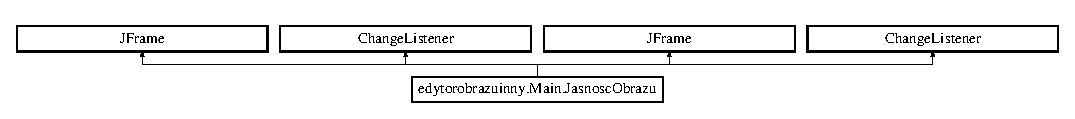
\includegraphics[height=1.147541cm]{classedytorobrazuinny_1_1_main_1_1_jasnosc_obrazu}
\end{center}
\end{figure}
\subsection*{Public Member Functions}
\begin{DoxyCompactItemize}
\item 
void \hyperlink{classedytorobrazuinny_1_1_main_1_1_jasnosc_obrazu_a7d3a28f2a8ff05803fd4e37e64452da5}{wylacz\+Slider} (boolean enabled)
\item 
void \hyperlink{classedytorobrazuinny_1_1_main_1_1_jasnosc_obrazu_a2783a21f72ef6067acbaa50136aa6c87}{state\+Changed} (Change\+Event e)
\item 
void \hyperlink{classedytorobrazuinny_1_1_main_1_1_jasnosc_obrazu_a7d3a28f2a8ff05803fd4e37e64452da5}{wylacz\+Slider} (boolean enabled)
\item 
void \hyperlink{classedytorobrazuinny_1_1_main_1_1_jasnosc_obrazu_a2783a21f72ef6067acbaa50136aa6c87}{state\+Changed} (Change\+Event e)
\end{DoxyCompactItemize}


\subsection{Member Function Documentation}
\hypertarget{classedytorobrazuinny_1_1_main_1_1_jasnosc_obrazu_a2783a21f72ef6067acbaa50136aa6c87}{}\index{edytorobrazuinny\+::\+Main\+::\+Jasnosc\+Obrazu@{edytorobrazuinny\+::\+Main\+::\+Jasnosc\+Obrazu}!state\+Changed@{state\+Changed}}
\index{state\+Changed@{state\+Changed}!edytorobrazuinny\+::\+Main\+::\+Jasnosc\+Obrazu@{edytorobrazuinny\+::\+Main\+::\+Jasnosc\+Obrazu}}
\subsubsection[{state\+Changed}]{\setlength{\rightskip}{0pt plus 5cm}void edytorobrazuinny.\+Main.\+Jasnosc\+Obrazu.\+state\+Changed (
\begin{DoxyParamCaption}
\item[{Change\+Event}]{e}
\end{DoxyParamCaption}
)}\label{classedytorobrazuinny_1_1_main_1_1_jasnosc_obrazu_a2783a21f72ef6067acbaa50136aa6c87}
\hypertarget{classedytorobrazuinny_1_1_main_1_1_jasnosc_obrazu_a2783a21f72ef6067acbaa50136aa6c87}{}\index{edytorobrazuinny\+::\+Main\+::\+Jasnosc\+Obrazu@{edytorobrazuinny\+::\+Main\+::\+Jasnosc\+Obrazu}!state\+Changed@{state\+Changed}}
\index{state\+Changed@{state\+Changed}!edytorobrazuinny\+::\+Main\+::\+Jasnosc\+Obrazu@{edytorobrazuinny\+::\+Main\+::\+Jasnosc\+Obrazu}}
\subsubsection[{state\+Changed}]{\setlength{\rightskip}{0pt plus 5cm}void edytorobrazuinny.\+Main.\+Jasnosc\+Obrazu.\+state\+Changed (
\begin{DoxyParamCaption}
\item[{Change\+Event}]{e}
\end{DoxyParamCaption}
)}\label{classedytorobrazuinny_1_1_main_1_1_jasnosc_obrazu_a2783a21f72ef6067acbaa50136aa6c87}
\hypertarget{classedytorobrazuinny_1_1_main_1_1_jasnosc_obrazu_a7d3a28f2a8ff05803fd4e37e64452da5}{}\index{edytorobrazuinny\+::\+Main\+::\+Jasnosc\+Obrazu@{edytorobrazuinny\+::\+Main\+::\+Jasnosc\+Obrazu}!wylacz\+Slider@{wylacz\+Slider}}
\index{wylacz\+Slider@{wylacz\+Slider}!edytorobrazuinny\+::\+Main\+::\+Jasnosc\+Obrazu@{edytorobrazuinny\+::\+Main\+::\+Jasnosc\+Obrazu}}
\subsubsection[{wylacz\+Slider}]{\setlength{\rightskip}{0pt plus 5cm}void edytorobrazuinny.\+Main.\+Jasnosc\+Obrazu.\+wylacz\+Slider (
\begin{DoxyParamCaption}
\item[{boolean}]{enabled}
\end{DoxyParamCaption}
)}\label{classedytorobrazuinny_1_1_main_1_1_jasnosc_obrazu_a7d3a28f2a8ff05803fd4e37e64452da5}
\hypertarget{classedytorobrazuinny_1_1_main_1_1_jasnosc_obrazu_a7d3a28f2a8ff05803fd4e37e64452da5}{}\index{edytorobrazuinny\+::\+Main\+::\+Jasnosc\+Obrazu@{edytorobrazuinny\+::\+Main\+::\+Jasnosc\+Obrazu}!wylacz\+Slider@{wylacz\+Slider}}
\index{wylacz\+Slider@{wylacz\+Slider}!edytorobrazuinny\+::\+Main\+::\+Jasnosc\+Obrazu@{edytorobrazuinny\+::\+Main\+::\+Jasnosc\+Obrazu}}
\subsubsection[{wylacz\+Slider}]{\setlength{\rightskip}{0pt plus 5cm}void edytorobrazuinny.\+Main.\+Jasnosc\+Obrazu.\+wylacz\+Slider (
\begin{DoxyParamCaption}
\item[{boolean}]{enabled}
\end{DoxyParamCaption}
)}\label{classedytorobrazuinny_1_1_main_1_1_jasnosc_obrazu_a7d3a28f2a8ff05803fd4e37e64452da5}


The documentation for this class was generated from the following file\+:\begin{DoxyCompactItemize}
\item 
\hyperlink{edytorobrazu_8java}{edytorobrazu.\+java}\end{DoxyCompactItemize}

\hypertarget{classedytorobrazuinny_1_1_main_1_1_skaluj_obraz_1_1_key_list}{}\section{edytorobrazuinny.\+Main.\+Skaluj\+Obraz.\+Key\+List Class Reference}
\label{classedytorobrazuinny_1_1_main_1_1_skaluj_obraz_1_1_key_list}\index{edytorobrazuinny.\+Main.\+Skaluj\+Obraz.\+Key\+List@{edytorobrazuinny.\+Main.\+Skaluj\+Obraz.\+Key\+List}}
Inheritance diagram for edytorobrazuinny.\+Main.\+Skaluj\+Obraz.\+Key\+List\+:\begin{figure}[H]
\begin{center}
\leavevmode
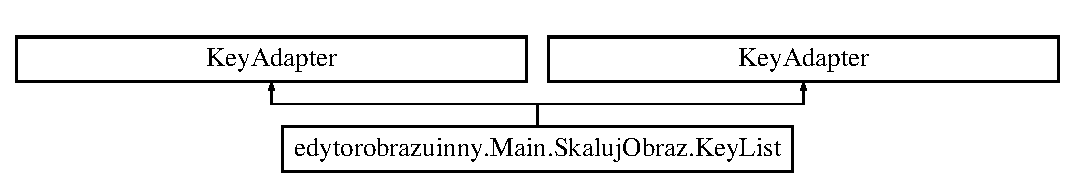
\includegraphics[height=2.000000cm]{classedytorobrazuinny_1_1_main_1_1_skaluj_obraz_1_1_key_list}
\end{center}
\end{figure}
\subsection*{Public Member Functions}
\begin{DoxyCompactItemize}
\item 
void \hyperlink{classedytorobrazuinny_1_1_main_1_1_skaluj_obraz_1_1_key_list_aba1533c6df2a8c3d4d0c0c4a682bdc35}{key\+Typed} (Key\+Event ke)
\item 
void \hyperlink{classedytorobrazuinny_1_1_main_1_1_skaluj_obraz_1_1_key_list_aba1533c6df2a8c3d4d0c0c4a682bdc35}{key\+Typed} (Key\+Event ke)
\end{DoxyCompactItemize}


\subsection{Member Function Documentation}
\hypertarget{classedytorobrazuinny_1_1_main_1_1_skaluj_obraz_1_1_key_list_aba1533c6df2a8c3d4d0c0c4a682bdc35}{}\index{edytorobrazuinny\+::\+Main\+::\+Skaluj\+Obraz\+::\+Key\+List@{edytorobrazuinny\+::\+Main\+::\+Skaluj\+Obraz\+::\+Key\+List}!key\+Typed@{key\+Typed}}
\index{key\+Typed@{key\+Typed}!edytorobrazuinny\+::\+Main\+::\+Skaluj\+Obraz\+::\+Key\+List@{edytorobrazuinny\+::\+Main\+::\+Skaluj\+Obraz\+::\+Key\+List}}
\subsubsection[{key\+Typed}]{\setlength{\rightskip}{0pt plus 5cm}void edytorobrazuinny.\+Main.\+Skaluj\+Obraz.\+Key\+List.\+key\+Typed (
\begin{DoxyParamCaption}
\item[{Key\+Event}]{ke}
\end{DoxyParamCaption}
)}\label{classedytorobrazuinny_1_1_main_1_1_skaluj_obraz_1_1_key_list_aba1533c6df2a8c3d4d0c0c4a682bdc35}
\hypertarget{classedytorobrazuinny_1_1_main_1_1_skaluj_obraz_1_1_key_list_aba1533c6df2a8c3d4d0c0c4a682bdc35}{}\index{edytorobrazuinny\+::\+Main\+::\+Skaluj\+Obraz\+::\+Key\+List@{edytorobrazuinny\+::\+Main\+::\+Skaluj\+Obraz\+::\+Key\+List}!key\+Typed@{key\+Typed}}
\index{key\+Typed@{key\+Typed}!edytorobrazuinny\+::\+Main\+::\+Skaluj\+Obraz\+::\+Key\+List@{edytorobrazuinny\+::\+Main\+::\+Skaluj\+Obraz\+::\+Key\+List}}
\subsubsection[{key\+Typed}]{\setlength{\rightskip}{0pt plus 5cm}void edytorobrazuinny.\+Main.\+Skaluj\+Obraz.\+Key\+List.\+key\+Typed (
\begin{DoxyParamCaption}
\item[{Key\+Event}]{ke}
\end{DoxyParamCaption}
)}\label{classedytorobrazuinny_1_1_main_1_1_skaluj_obraz_1_1_key_list_aba1533c6df2a8c3d4d0c0c4a682bdc35}


The documentation for this class was generated from the following file\+:\begin{DoxyCompactItemize}
\item 
\hyperlink{edytorobrazu_8java}{edytorobrazu.\+java}\end{DoxyCompactItemize}

\hypertarget{classedytorobrazuinny_1_1_main_1_1_skaluj_obraz}{}\section{edytorobrazuinny.\+Main.\+Skaluj\+Obraz Class Reference}
\label{classedytorobrazuinny_1_1_main_1_1_skaluj_obraz}\index{edytorobrazuinny.\+Main.\+Skaluj\+Obraz@{edytorobrazuinny.\+Main.\+Skaluj\+Obraz}}
Inheritance diagram for edytorobrazuinny.\+Main.\+Skaluj\+Obraz\+:\begin{figure}[H]
\begin{center}
\leavevmode
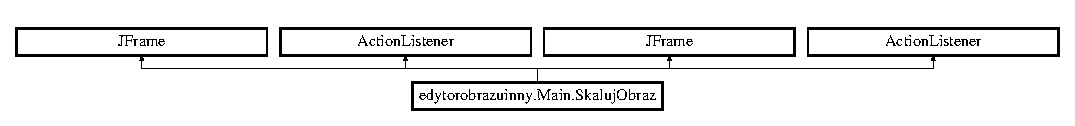
\includegraphics[height=1.250000cm]{classedytorobrazuinny_1_1_main_1_1_skaluj_obraz}
\end{center}
\end{figure}
\subsection*{Classes}
\begin{DoxyCompactItemize}
\item 
class \hyperlink{classedytorobrazuinny_1_1_main_1_1_skaluj_obraz_1_1_key_list}{Key\+List}
\end{DoxyCompactItemize}
\subsection*{Public Member Functions}
\begin{DoxyCompactItemize}
\item 
void \hyperlink{classedytorobrazuinny_1_1_main_1_1_skaluj_obraz_ab796d938ac3680ee7b2aaf991cae3e95}{wylacz\+Komponenty} (boolean enabled)
\item 
void \hyperlink{classedytorobrazuinny_1_1_main_1_1_skaluj_obraz_a7422a35e2ee09b44bdd4ecaee0cf58f9}{action\+Performed} (Action\+Event e)
\item 
void \hyperlink{classedytorobrazuinny_1_1_main_1_1_skaluj_obraz_ab796d938ac3680ee7b2aaf991cae3e95}{wylacz\+Komponenty} (boolean enabled)
\item 
void \hyperlink{classedytorobrazuinny_1_1_main_1_1_skaluj_obraz_a7422a35e2ee09b44bdd4ecaee0cf58f9}{action\+Performed} (Action\+Event e)
\end{DoxyCompactItemize}


\subsection{Member Function Documentation}
\hypertarget{classedytorobrazuinny_1_1_main_1_1_skaluj_obraz_a7422a35e2ee09b44bdd4ecaee0cf58f9}{}\index{edytorobrazuinny\+::\+Main\+::\+Skaluj\+Obraz@{edytorobrazuinny\+::\+Main\+::\+Skaluj\+Obraz}!action\+Performed@{action\+Performed}}
\index{action\+Performed@{action\+Performed}!edytorobrazuinny\+::\+Main\+::\+Skaluj\+Obraz@{edytorobrazuinny\+::\+Main\+::\+Skaluj\+Obraz}}
\subsubsection[{action\+Performed}]{\setlength{\rightskip}{0pt plus 5cm}void edytorobrazuinny.\+Main.\+Skaluj\+Obraz.\+action\+Performed (
\begin{DoxyParamCaption}
\item[{Action\+Event}]{e}
\end{DoxyParamCaption}
)}\label{classedytorobrazuinny_1_1_main_1_1_skaluj_obraz_a7422a35e2ee09b44bdd4ecaee0cf58f9}
\hypertarget{classedytorobrazuinny_1_1_main_1_1_skaluj_obraz_a7422a35e2ee09b44bdd4ecaee0cf58f9}{}\index{edytorobrazuinny\+::\+Main\+::\+Skaluj\+Obraz@{edytorobrazuinny\+::\+Main\+::\+Skaluj\+Obraz}!action\+Performed@{action\+Performed}}
\index{action\+Performed@{action\+Performed}!edytorobrazuinny\+::\+Main\+::\+Skaluj\+Obraz@{edytorobrazuinny\+::\+Main\+::\+Skaluj\+Obraz}}
\subsubsection[{action\+Performed}]{\setlength{\rightskip}{0pt plus 5cm}void edytorobrazuinny.\+Main.\+Skaluj\+Obraz.\+action\+Performed (
\begin{DoxyParamCaption}
\item[{Action\+Event}]{e}
\end{DoxyParamCaption}
)}\label{classedytorobrazuinny_1_1_main_1_1_skaluj_obraz_a7422a35e2ee09b44bdd4ecaee0cf58f9}
\hypertarget{classedytorobrazuinny_1_1_main_1_1_skaluj_obraz_ab796d938ac3680ee7b2aaf991cae3e95}{}\index{edytorobrazuinny\+::\+Main\+::\+Skaluj\+Obraz@{edytorobrazuinny\+::\+Main\+::\+Skaluj\+Obraz}!wylacz\+Komponenty@{wylacz\+Komponenty}}
\index{wylacz\+Komponenty@{wylacz\+Komponenty}!edytorobrazuinny\+::\+Main\+::\+Skaluj\+Obraz@{edytorobrazuinny\+::\+Main\+::\+Skaluj\+Obraz}}
\subsubsection[{wylacz\+Komponenty}]{\setlength{\rightskip}{0pt plus 5cm}void edytorobrazuinny.\+Main.\+Skaluj\+Obraz.\+wylacz\+Komponenty (
\begin{DoxyParamCaption}
\item[{boolean}]{enabled}
\end{DoxyParamCaption}
)}\label{classedytorobrazuinny_1_1_main_1_1_skaluj_obraz_ab796d938ac3680ee7b2aaf991cae3e95}
\hypertarget{classedytorobrazuinny_1_1_main_1_1_skaluj_obraz_ab796d938ac3680ee7b2aaf991cae3e95}{}\index{edytorobrazuinny\+::\+Main\+::\+Skaluj\+Obraz@{edytorobrazuinny\+::\+Main\+::\+Skaluj\+Obraz}!wylacz\+Komponenty@{wylacz\+Komponenty}}
\index{wylacz\+Komponenty@{wylacz\+Komponenty}!edytorobrazuinny\+::\+Main\+::\+Skaluj\+Obraz@{edytorobrazuinny\+::\+Main\+::\+Skaluj\+Obraz}}
\subsubsection[{wylacz\+Komponenty}]{\setlength{\rightskip}{0pt plus 5cm}void edytorobrazuinny.\+Main.\+Skaluj\+Obraz.\+wylacz\+Komponenty (
\begin{DoxyParamCaption}
\item[{boolean}]{enabled}
\end{DoxyParamCaption}
)}\label{classedytorobrazuinny_1_1_main_1_1_skaluj_obraz_ab796d938ac3680ee7b2aaf991cae3e95}


The documentation for this class was generated from the following file\+:\begin{DoxyCompactItemize}
\item 
\hyperlink{edytorobrazu_8java}{edytorobrazu.\+java}\end{DoxyCompactItemize}

\hypertarget{classedytorobrazuinny_1_1_main_1_1_tekst_dodaj}{}\section{edytorobrazuinny.\+Main.\+Tekst\+Dodaj Class Reference}
\label{classedytorobrazuinny_1_1_main_1_1_tekst_dodaj}\index{edytorobrazuinny.\+Main.\+Tekst\+Dodaj@{edytorobrazuinny.\+Main.\+Tekst\+Dodaj}}
Inheritance diagram for edytorobrazuinny.\+Main.\+Tekst\+Dodaj\+:\begin{figure}[H]
\begin{center}
\leavevmode
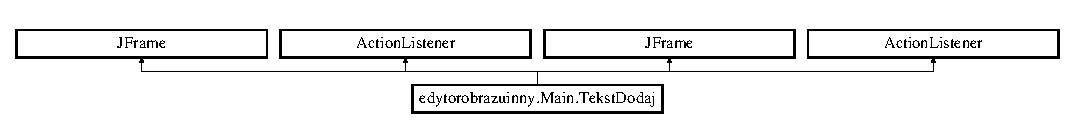
\includegraphics[height=1.290323cm]{classedytorobrazuinny_1_1_main_1_1_tekst_dodaj}
\end{center}
\end{figure}
\subsection*{Public Member Functions}
\begin{DoxyCompactItemize}
\item 
void \hyperlink{classedytorobrazuinny_1_1_main_1_1_tekst_dodaj_a3752cac64a494056099893a07622965a}{action\+Performed} (Action\+Event e)
\item 
void \hyperlink{classedytorobrazuinny_1_1_main_1_1_tekst_dodaj_a0105a0926695972cf4345e090436a9b9}{list\+Fonts} ()
\item 
void \hyperlink{classedytorobrazuinny_1_1_main_1_1_tekst_dodaj_a3752cac64a494056099893a07622965a}{action\+Performed} (Action\+Event e)
\item 
void \hyperlink{classedytorobrazuinny_1_1_main_1_1_tekst_dodaj_a0105a0926695972cf4345e090436a9b9}{list\+Fonts} ()
\end{DoxyCompactItemize}


\subsection{Member Function Documentation}
\hypertarget{classedytorobrazuinny_1_1_main_1_1_tekst_dodaj_a3752cac64a494056099893a07622965a}{}\index{edytorobrazuinny\+::\+Main\+::\+Tekst\+Dodaj@{edytorobrazuinny\+::\+Main\+::\+Tekst\+Dodaj}!action\+Performed@{action\+Performed}}
\index{action\+Performed@{action\+Performed}!edytorobrazuinny\+::\+Main\+::\+Tekst\+Dodaj@{edytorobrazuinny\+::\+Main\+::\+Tekst\+Dodaj}}
\subsubsection[{action\+Performed}]{\setlength{\rightskip}{0pt plus 5cm}void edytorobrazuinny.\+Main.\+Tekst\+Dodaj.\+action\+Performed (
\begin{DoxyParamCaption}
\item[{Action\+Event}]{e}
\end{DoxyParamCaption}
)}\label{classedytorobrazuinny_1_1_main_1_1_tekst_dodaj_a3752cac64a494056099893a07622965a}
\hypertarget{classedytorobrazuinny_1_1_main_1_1_tekst_dodaj_a3752cac64a494056099893a07622965a}{}\index{edytorobrazuinny\+::\+Main\+::\+Tekst\+Dodaj@{edytorobrazuinny\+::\+Main\+::\+Tekst\+Dodaj}!action\+Performed@{action\+Performed}}
\index{action\+Performed@{action\+Performed}!edytorobrazuinny\+::\+Main\+::\+Tekst\+Dodaj@{edytorobrazuinny\+::\+Main\+::\+Tekst\+Dodaj}}
\subsubsection[{action\+Performed}]{\setlength{\rightskip}{0pt plus 5cm}void edytorobrazuinny.\+Main.\+Tekst\+Dodaj.\+action\+Performed (
\begin{DoxyParamCaption}
\item[{Action\+Event}]{e}
\end{DoxyParamCaption}
)}\label{classedytorobrazuinny_1_1_main_1_1_tekst_dodaj_a3752cac64a494056099893a07622965a}
\hypertarget{classedytorobrazuinny_1_1_main_1_1_tekst_dodaj_a0105a0926695972cf4345e090436a9b9}{}\index{edytorobrazuinny\+::\+Main\+::\+Tekst\+Dodaj@{edytorobrazuinny\+::\+Main\+::\+Tekst\+Dodaj}!list\+Fonts@{list\+Fonts}}
\index{list\+Fonts@{list\+Fonts}!edytorobrazuinny\+::\+Main\+::\+Tekst\+Dodaj@{edytorobrazuinny\+::\+Main\+::\+Tekst\+Dodaj}}
\subsubsection[{list\+Fonts}]{\setlength{\rightskip}{0pt plus 5cm}void edytorobrazuinny.\+Main.\+Tekst\+Dodaj.\+list\+Fonts (
\begin{DoxyParamCaption}
{}
\end{DoxyParamCaption}
)}\label{classedytorobrazuinny_1_1_main_1_1_tekst_dodaj_a0105a0926695972cf4345e090436a9b9}
\hypertarget{classedytorobrazuinny_1_1_main_1_1_tekst_dodaj_a0105a0926695972cf4345e090436a9b9}{}\index{edytorobrazuinny\+::\+Main\+::\+Tekst\+Dodaj@{edytorobrazuinny\+::\+Main\+::\+Tekst\+Dodaj}!list\+Fonts@{list\+Fonts}}
\index{list\+Fonts@{list\+Fonts}!edytorobrazuinny\+::\+Main\+::\+Tekst\+Dodaj@{edytorobrazuinny\+::\+Main\+::\+Tekst\+Dodaj}}
\subsubsection[{list\+Fonts}]{\setlength{\rightskip}{0pt plus 5cm}void edytorobrazuinny.\+Main.\+Tekst\+Dodaj.\+list\+Fonts (
\begin{DoxyParamCaption}
{}
\end{DoxyParamCaption}
)}\label{classedytorobrazuinny_1_1_main_1_1_tekst_dodaj_a0105a0926695972cf4345e090436a9b9}


The documentation for this class was generated from the following file\+:\begin{DoxyCompactItemize}
\item 
\hyperlink{edytorobrazu_8java}{edytorobrazu.\+java}\end{DoxyCompactItemize}

\chapter{File Documentation}
\hypertarget{edytorobrazu_8java}{}\section{edytorobrazu.\+java File Reference}
\label{edytorobrazu_8java}\index{edytorobrazu.\+java@{edytorobrazu.\+java}}
\subsection*{Classes}
\begin{DoxyCompactItemize}
\item 
class {\bfseries edytorobrazuinny.\+Img\+Area}
\item 
class {\bfseries edytorobrazuinny.\+Img\+Area.\+Mousexy}
\item 
class {\bfseries edytorobrazuinny.\+Img\+Area.\+K\+List}
\item 
class {\bfseries edytorobrazuinny.\+Main}
\item 
class \hyperlink{classedytorobrazuinny_1_1_main_1_1_jasnosc_obrazu}{edytorobrazuinny.\+Main.\+Jasnosc\+Obrazu}
\item 
class \hyperlink{classedytorobrazuinny_1_1_main_1_1_skaluj_obraz}{edytorobrazuinny.\+Main.\+Skaluj\+Obraz}
\item 
class \hyperlink{classedytorobrazuinny_1_1_main_1_1_skaluj_obraz_1_1_key_list}{edytorobrazuinny.\+Main.\+Skaluj\+Obraz.\+Key\+List}
\item 
class \hyperlink{classedytorobrazuinny_1_1_main_1_1_tekst_dodaj}{edytorobrazuinny.\+Main.\+Tekst\+Dodaj}
\item 
class \hyperlink{classedytorobrazuinny_1_1edytorobrazu}{edytorobrazuinny.\+edytorobrazu}
\end{DoxyCompactItemize}
\subsection*{Packages}
\begin{DoxyCompactItemize}
\item 
package \hyperlink{namespaceedytorobrazuinny}{edytorobrazuinny}
\end{DoxyCompactItemize}

\hypertarget{_edytor_obrazu_inny_2src_2edytorobrazuinny_2edytorobrazu_8java}{}\section{Edytor\+Obrazu\+Inny/src/edytorobrazuinny/edytorobrazu.java File Reference}
\label{_edytor_obrazu_inny_2src_2edytorobrazuinny_2edytorobrazu_8java}\index{Edytor\+Obrazu\+Inny/src/edytorobrazuinny/edytorobrazu.\+java@{Edytor\+Obrazu\+Inny/src/edytorobrazuinny/edytorobrazu.\+java}}
\subsection*{Classes}
\begin{DoxyCompactItemize}
\item 
class {\bfseries edytorobrazuinny.\+Img\+Area}
\item 
class {\bfseries edytorobrazuinny.\+Img\+Area.\+Mousexy}
\item 
class {\bfseries edytorobrazuinny.\+Img\+Area.\+K\+List}
\item 
class {\bfseries edytorobrazuinny.\+Main}
\item 
class \hyperlink{classedytorobrazuinny_1_1_main_1_1_jasnosc_obrazu}{edytorobrazuinny.\+Main.\+Jasnosc\+Obrazu}
\item 
class \hyperlink{classedytorobrazuinny_1_1_main_1_1_skaluj_obraz}{edytorobrazuinny.\+Main.\+Skaluj\+Obraz}
\item 
class \hyperlink{classedytorobrazuinny_1_1_main_1_1_skaluj_obraz_1_1_key_list}{edytorobrazuinny.\+Main.\+Skaluj\+Obraz.\+Key\+List}
\item 
class \hyperlink{classedytorobrazuinny_1_1_main_1_1_tekst_dodaj}{edytorobrazuinny.\+Main.\+Tekst\+Dodaj}
\item 
class \hyperlink{classedytorobrazuinny_1_1edytorobrazu}{edytorobrazuinny.\+edytorobrazu}
\end{DoxyCompactItemize}
\subsection*{Packages}
\begin{DoxyCompactItemize}
\item 
package \hyperlink{namespaceedytorobrazuinny}{edytorobrazuinny}
\end{DoxyCompactItemize}

%--- End generated contents ---

% Index
\backmatter
\newpage
\phantomsection
\clearemptydoublepage
\addcontentsline{toc}{chapter}{Index}
\printindex

\end{document}
